
The goal of this thesis was to gauge the fault tolerance of approximate computing tools using software fault injection. Hardware fault injection is prohibitively expensive and difficult, while software fault injection can also emulate hardware faults in addition to injecting developmental faults. The fault injection was performed in LLVM bytecode in an effort to make the results applicable regardless of programming language and to create the groundwork for the creation of an automated fault injection pass that can be created as further work.

The tools that were tested were \floatsmith{} and \taffo{}.

\section{Installation}
Prerequisite to testing the tools is installing the tools. \taffo{} depends on LLVM 14 or 15 to run, and is at the time of writing not compatible with newer versions of LLVM (the most recent version is LLVM 20). LLVM 15 can be built from the source code following the instructions found at the LLVM website, \url{llvm.org}. On certain GNU/linux distributions you may also install LLVM through your package manager (if supported by the LLVM organization), but you may need to add the LLVM repository  to your package manager of choice for this to work. 

Building \taffo{} was successful when using pre-built LLVM binaries. 
The other tool that was used was \floatsmith ~\citep{floatsmith_paper}. This can be installed the easiest using their provided docker image, and mounting the project you want to perform experiments on within the docker image.

\section{Bitwise fault injection}\label{section:bitwise_fault_injection}
Bitwise fault injection was done through manually performing an XOR (exclusive or) operation in LLVM bytecode on the values to be subjected to faults. Table~\ref{table:xor_truth_table} shows the truth table for two bit inputs through an XOR-gate. The output is 1 if and only if either input A or input B is 1 while the other is 0. If using input B as a bit mask of which bits to flip, we can see in the table that the output becomes the opposite of input A for all cases of input B being 1, and when input B is 0 all outputs are the same as input A, allowing us to flip a single bit at a time. An XOR operation on two 8-bit numbers is shown in figure~\ref{fig:xor_operation}. The output of the XOR operation shows that the output is the same as the input, except for the bit that is marked with red, which has been flipped.

\begin{table}[htb]
    \centering
\caption{Truth table for XOR function}
    \label{table:xor_truth_table}
\begin{tabular}{c|c|c}
     input A& input B& XOR output \\
     0&0&0\\
     1&0&1\\
     0&1&1\\
     1&1&0
\end{tabular}
    
\end{table}



\begin{figure}[h!]
    \centering
    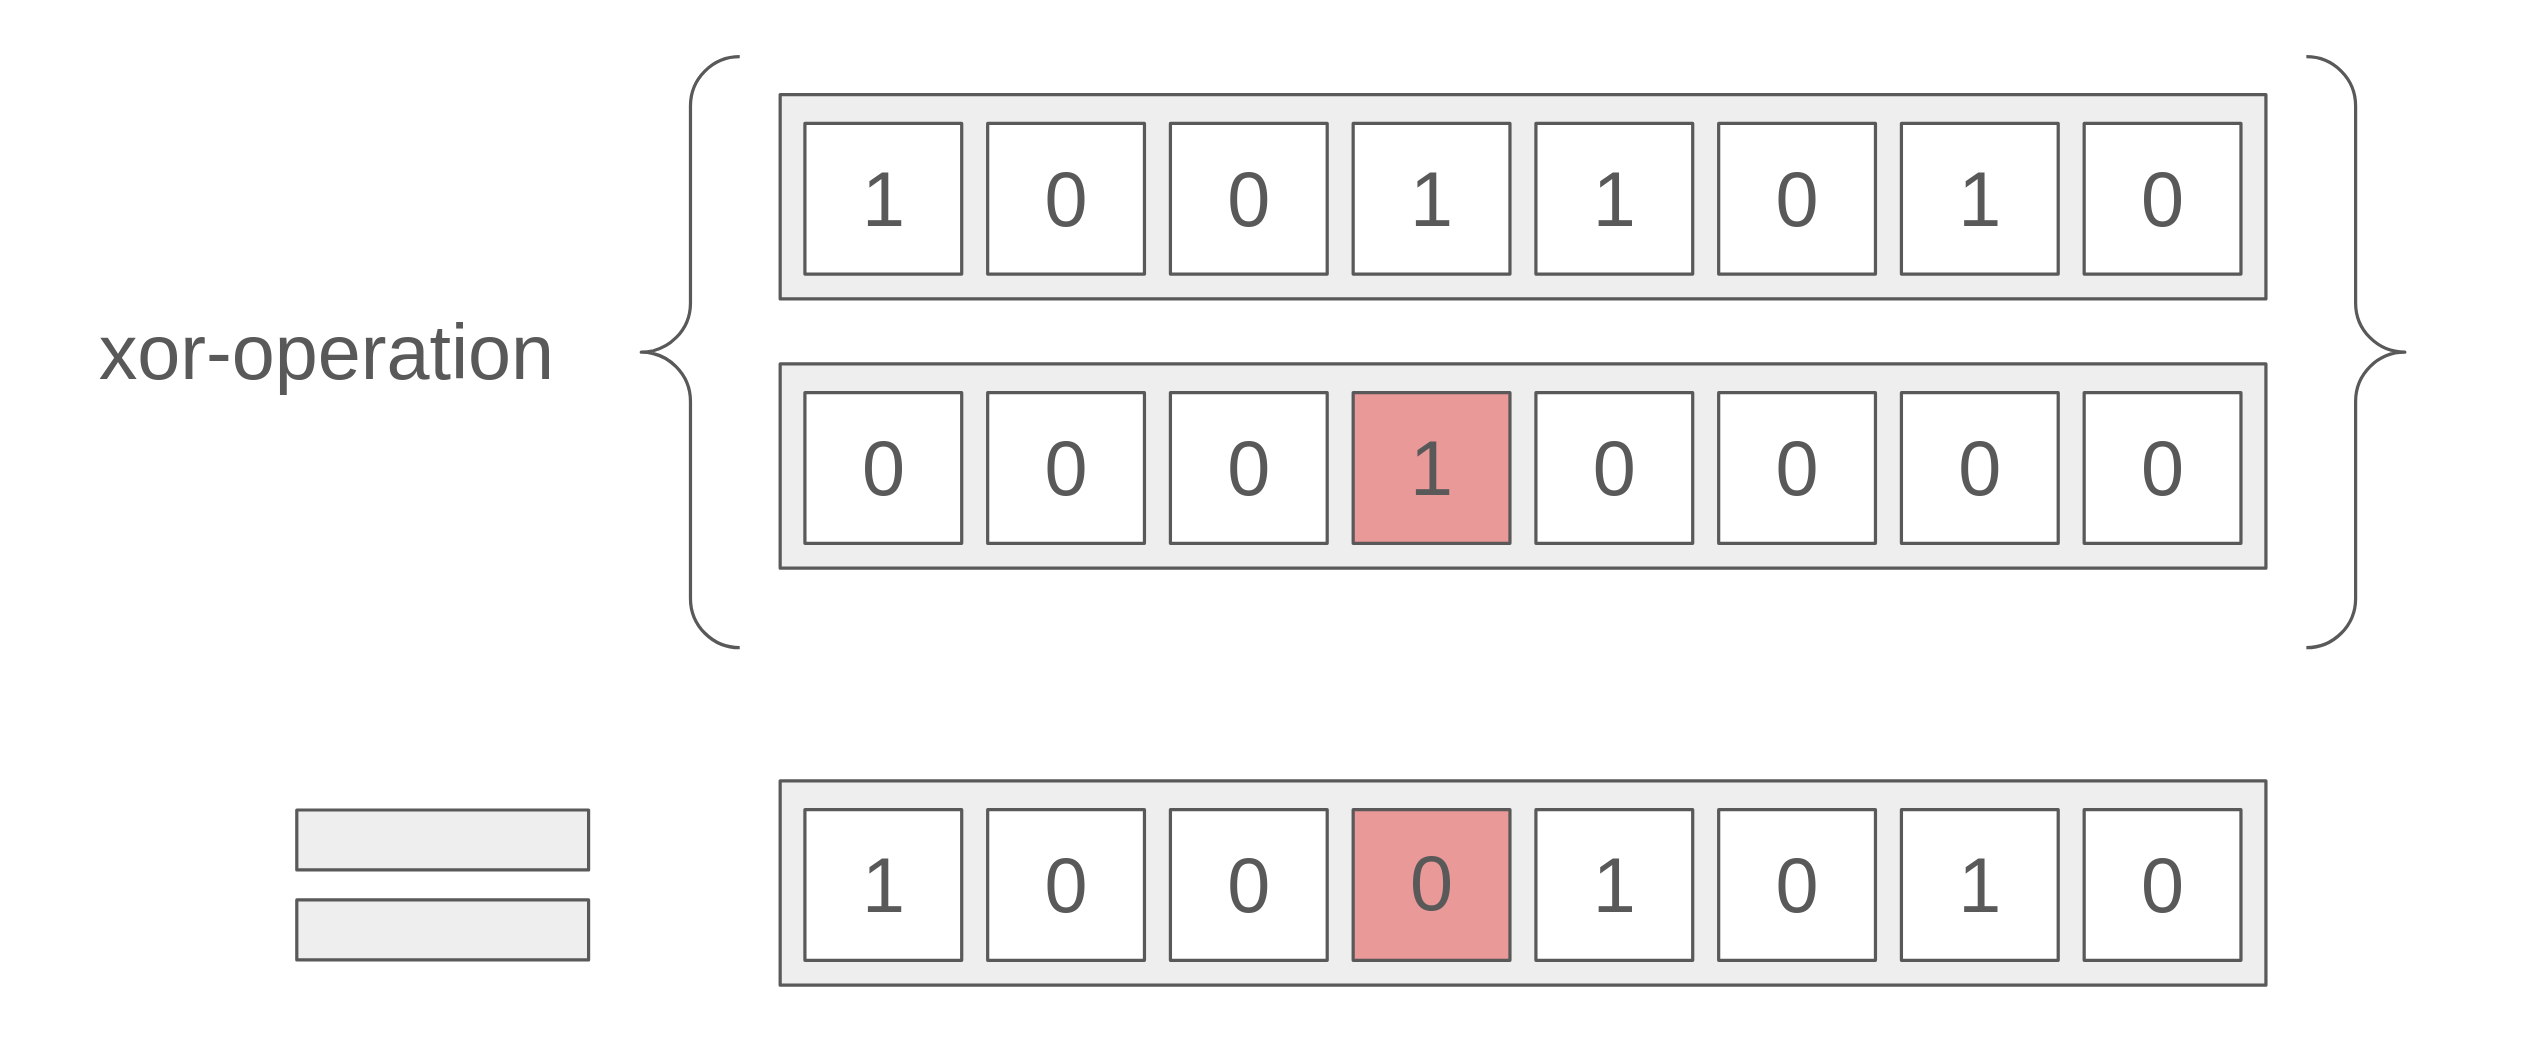
\includegraphics[width=0.75\linewidth]{Images/xor_operation.png}
    \caption{An example XOR operation between two numbers.}
    \label{fig:xor_operation}
\end{figure}

This was applied directly in LLVM bytecode using LLVM bytecode commands to perform a bit flip on a data variable in the program. Code listing~\ref{listing:llvm_ir_fixed} shows how the bit flip was implemented for the fixed point implementation, and listing~\ref{listing:llvm_ir_float} shows the bit flip for the floating point implementation.



The result of a division is selected as the value to perform fault injection on as there are only two division operations in the selected benchmark's source code, one in the data generation part of the code, and one in the main computational kernel. These two division operations can be distinguished from each other through the fact that the division in the main computational kernel divides a variable by the constant value 9. This constant value is preserved directly in LLVM bytecode, which makes it trivial to find the division operation in the data preparation function.\footnote{The fixed point implementation bytecode actually contains three division operations, of which one is a floating point division. This is suspected to be dead code that isn't optimized away, but it is disregarded for this fault injection campaign.}
In addition to this, the function names are preserved, but it is tedious to traverse the function to find the instruction to be injected with an error. It is much easier just searching for the LLVM bytecode instruction {\tt fdiv} for floating point division and {\tt sdiv} for fixed point division in the respective implementations.

Two temporary variables, \%temp1 and \%temp2, are introduced, where \%temp1 is a 64 bit integer with value 1 shifted left however many bits necessary to inject a bit in the desired location. Listing~\ref{listing:llvm_ir_fixed} injects a bit in bit index number 4, making the last 8 bits of \%temp1 equivalent with the binary number (with the bit highlighted in red) shown in figure~\ref{fig:xor_operation}.
The variable \%temp2 stores the result of the XOR operation between the result of the division in the variable \%18 and the bit mask from \%temp1, and is then placed where variable \%18 ordinarily would be in the variable \%s10\_22fixp4.

\begin{lstlisting}[caption=fixed point bit flip in LLVM bytecode, label=listing:llvm_ir_fixed]
  %17 = sext i32 %0 to i64, !taffo.info !45
  %18 = sdiv i64 %16, %17, !taffo.info !109
  %temp1 = shl i64 1, 4
  %temp2 = xor i64 %temp1, %18
  %s10_22fixp4 = trunc i64 %temp2 to i32, !taffo.info !110
\end{lstlisting} 

\begin{lstlisting}[caption=floating point bit flip in LLVM bytecode, label=listing:llvm_ir_float]
  %temp1 = fdiv double %24, %26
  %temp2 = shl i64 1, 4
  %temp3 = bitcast double %temp1 to i64
  %temp4 = xor i64 %temp2, %temp3
  %27 = bitcast i64 %temp4 to double
\end{lstlisting}

Flipping a bit in the floating point implementation requires first performing a bitcast operation on the floating point number to be fault injected, \%temp1 in listing~\ref{listing:llvm_ir_float}. A bitcast is an operation that marks the bits in the memory location of \%temp1 as an integer, without actually changing any of the bits. This has to be done because the number 1 stored as a fixed point number is all zeros except the least significant bit which is 1, and a floating point binary representation contains several bits set to 1 in the exponent part of the number due to the exponent offset, see~\ref{section:approximate_computing_through_reducing_bits}. After the fault injection is performed, the fault injected variable then needs to be bitcast back to a floating point number.

The first fault injection campaign consisted of single bit fault injections within bytecode variables. This consisted of taking a sample benchmark from the \taffo{} repository, compiling it to LLVM bytecode, then flipping single bits one location at a time, and building it to a fault injected executable. This is possible because the data for the benchmarks are generated in the same file as the computational kernel that is benchmark in a loop. For each iteration of this loop, a bit is flipped in the result of one iteration, and the fault is injected for all iterations of the loop. For \taffo{}, which converts floating point values to lower precision fixed point values, this requires creating a fault injected version for both the fixed and floating point LLVM bytecode.

% For each pair of fault injected executables, the outputs are compared between each other and the original floating point implementation.

To streamline injections a helper script was created based on the existing scripts in the \taffo{} repository. This allows a user to compile the selected benchmark from a list of benchmarks to LLVM bytecode, inject faults in a user-selected location in the code, then change the bit location of this fault, and compile many different versions of the same benchmark with different faults injected in the same location. The script then runs all the benchmarks and collects output. Finally a python script that reads these outputs collects and compares them in a human readable format. To use the script, the user needs to manually set the range of bits that are being flipped in the run script. 

The comparison script written in python was written in a separate repository with tests, and iteratively copied over to the \taffo{} repository as development progressed. It was written to compare one single benchmark at a time, and this is documented in the repository. The comparison script is designed to only compare the results of the fault injection of a single benchmark at a time. See the appendix for the link to the repository.



% her skrive om mutation-isj testing i taffo

